\section{Virtual Group Room}
\label{sec:prePgrRom}
A screenshot of a virtual group room can be seen in \figref{fig:projectgroupnoedit}. 
In this virtual group room the blocks of the standard layout are seen.
\begin{figure}[h]
	\centering
		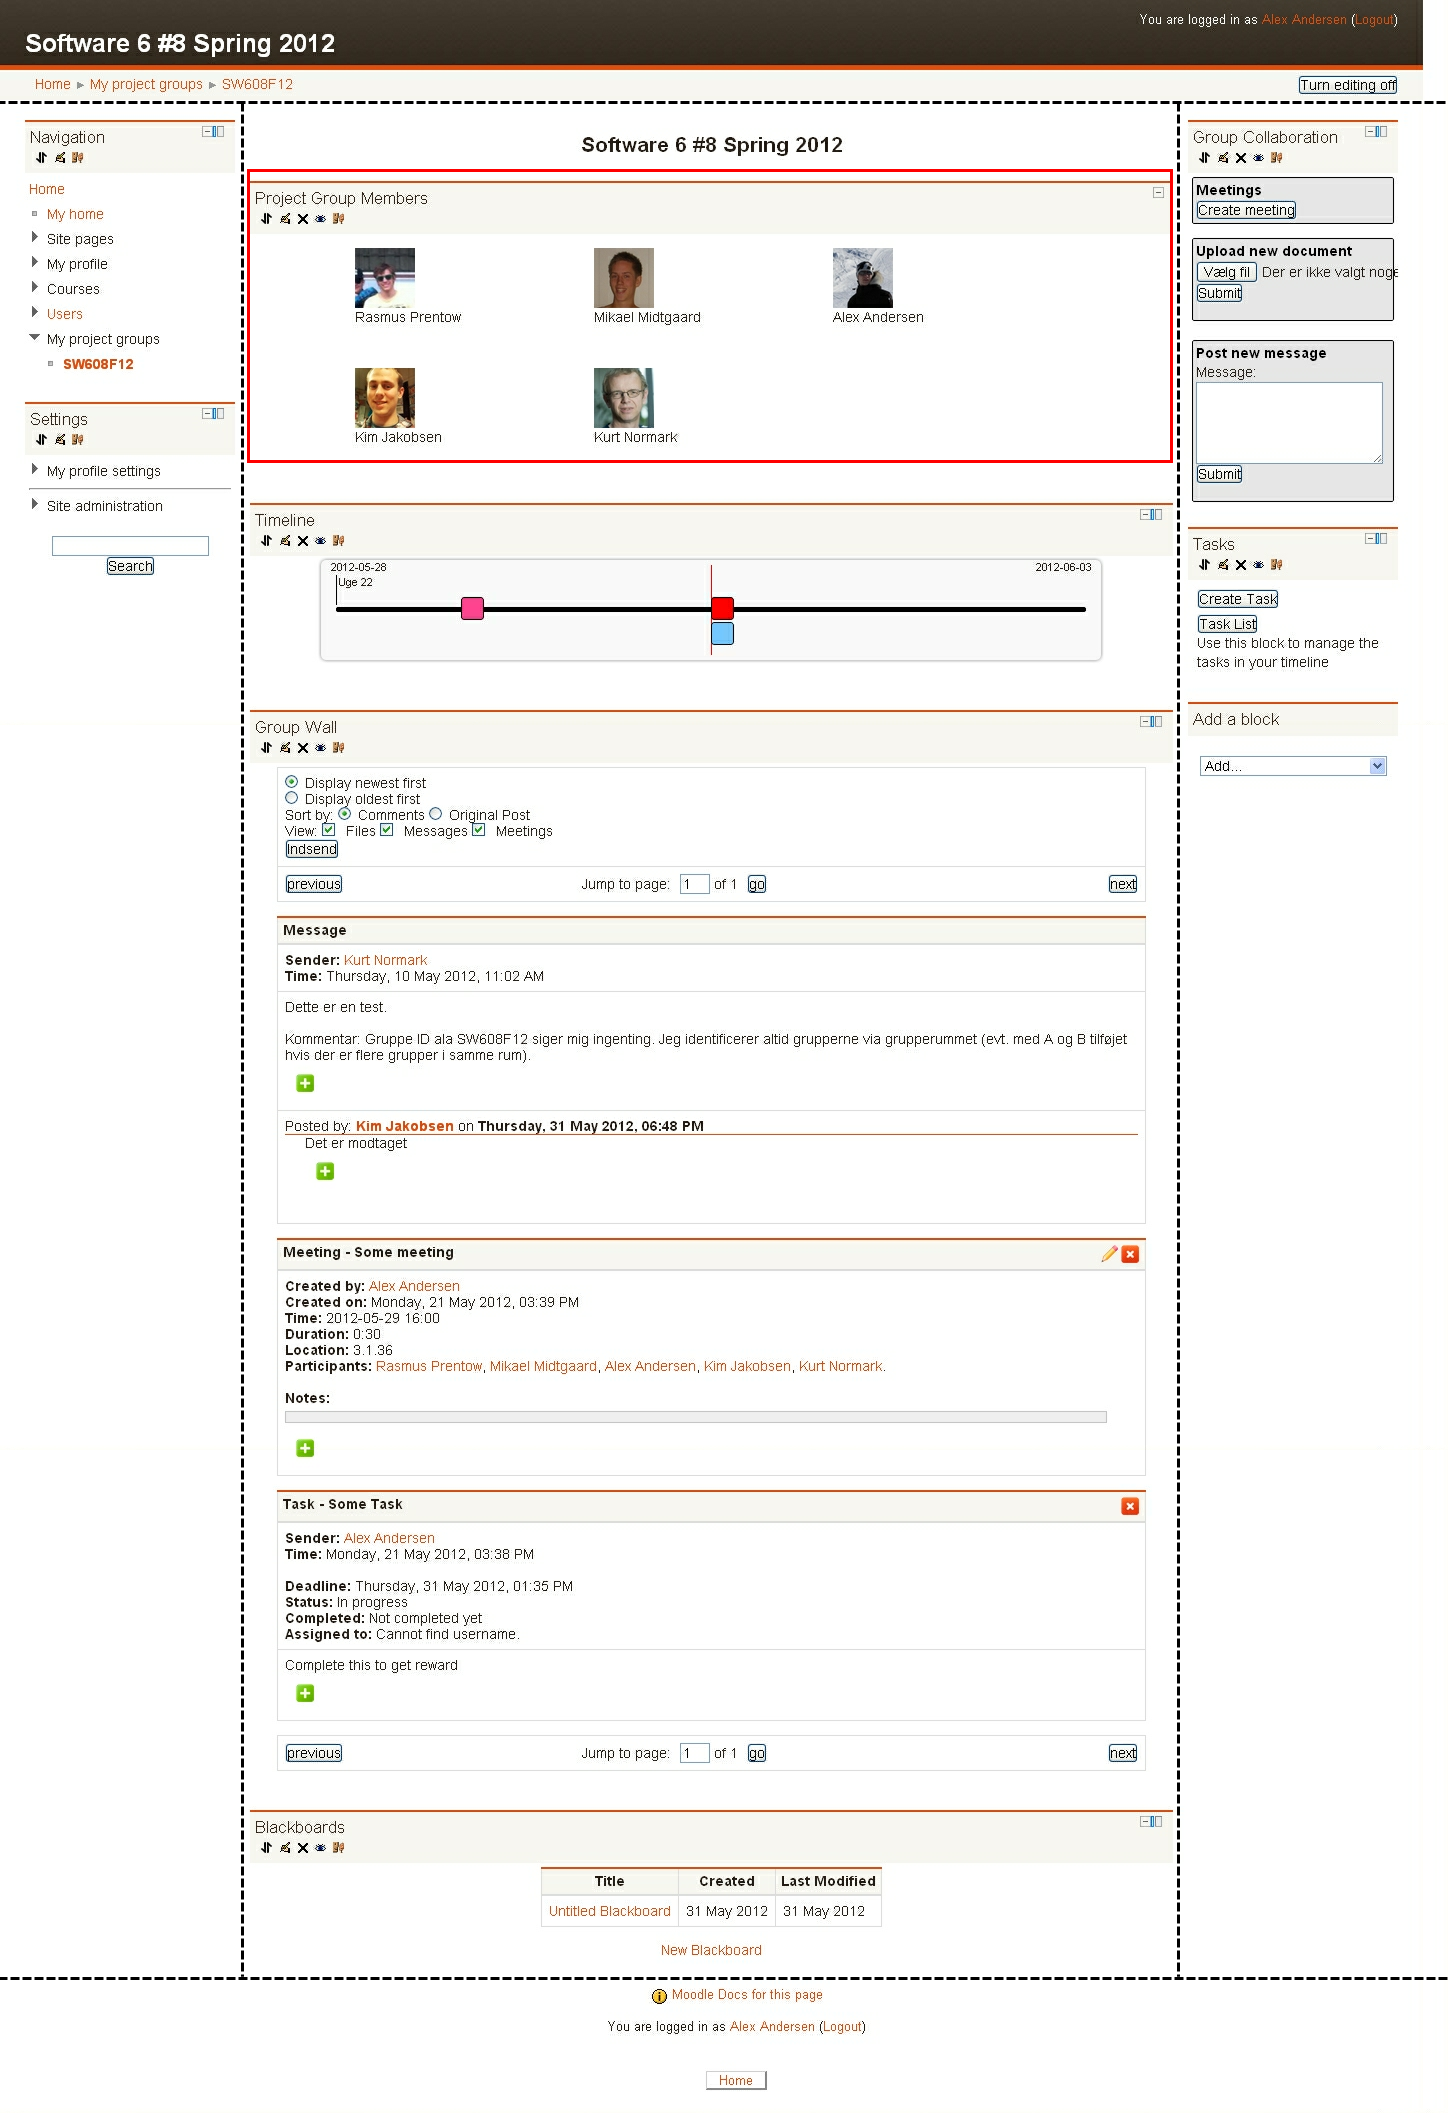
\includegraphics[width=\textwidth]{images/projectgroupnoedit2.png}
	\morscaption{The virtual group room. The highlighted box shows the project group block and the dashed lines show the different areas on the page}
	\label{fig:projectgroupnoedit}
\end{figure}

The virtual group room consists of three rows.
The screenshot illustrates the area boundaries by dashed lines. 
%An illustrationThe page in edit mode can be seen in figure \figref{fig:projectgroupwithedit}.
The three rows on the page are: The header, the middle, and the footer. 
%The header is standard Moodle and is only controlled by us to add a heading. 
The header is a standard Moodle component, and we affect it by adding a headline -- the rest of the header is added automatically.
The header shows the name of the project group. 
The middle part contains the content of the virtual group room, and it is divided into three columns. 
The left column contains the standard navigation block in Moodle and is not created by us, though it is extended by us.
%We do not want anything to be added to this column to ensure that the page seem familiar to the user.
The center and right columns both contain custom \block{}s.
The center area is much wider than the left and right and can therefore contain bigger \block{}s. 
The various \block{}s presented in the virtual group room are described in \secref{sec:implprojectgroupblocks}. 
If a user wants to edit the layout for the virtual group room he can press the ``Turn editing on'' button. 
This will allow the user to remove, add, move, and edit \block{}s. 
A special ``add new block''-block is added in editing mode to allow for adding new \block{}s. 
If a user edits the page, the change can be seen by all group members. 
Note that the virtual group room in \figref{fig:projectgroupnoedit} is in editing mode.

In the figure an example of a \block{} can be seen; it is denoted with a highlighted box.
The highlighted box contains the members block and is created by our sub-group; we elaborate on the implementation of this in \secref{sub:membersblock}. 
The block shows a photograph and the name of each member of the project group. 



